%%%%%%%%%%%%%%%%%%%%%%%%%%%%%%%%%%%%%%%%%
% University/School Laboratory Report
% LaTeX Template
% Version 3.1 (25/3/14)
%
% This template has been downloaded from:
% http://www.LaTeXTemplates.com
%
% Original author:
% Linux and Unix Users Group at Virginia Tech Wiki 
% (https://vtluug.org/wiki/Example_LaTeX_chem_lab_report)
%
% License:
% CC BY-NC-SA 3.0 (http://creativecommons.org/licenses/by-nc-sa/3.0/)
%
%%%%%%%%%%%%%%%%%%%%%%%%%%%%%%%%%%%%%%%%%

%----------------------------------------------------------------------------------------
%	PACKAGES AND DOCUMENT CONFIGURATIONS
%----------------------------------------------------------------------------------------

\documentclass{article}

\usepackage[version=3]{mhchem} % Package for chemical equation typesetting
\usepackage{siunitx} % Provides the \SI{}{} and \si{} command for typesetting SI units
\usepackage{graphicx} % Required for the inclusion of images
\usepackage{natbib} % Required to change bibliography style to APA
\usepackage{amsmath} % Required for some math elements 
\usepackage[utf8]{inputenc}
\usepackage{tikz,pgfplots}
\usepackage[letterpaper, margin=0.5in]{geometry}
\usepackage{float}
\usepackage{enumitem}
\usepackage{fixltx2e}
\usepackage{gensymb}
\usepackage[hidelinks]{hyperref}
\usepackage[all]{hypcap}
\usepackage{csvsimple}

\usepackage{xcolor}

% Roman numerials
\pagenumbering{arabic}

\setlength\parindent{0pt} % Removes all indentation from paragraphs

%\renewcommand{\labelenumi}{\alph{enumi}.} % Make numbering in the enumerate environment by letter rather than number (e.g. section 6)

%\usepackage{times} % Uncomment to use the Times New Roman font

% for some tables
\newcommand{\specialcell}[2][c]{%
  \begin{tabular}[#1]{@{}c@{}}#2\end{tabular}}
  
\providecommand{\e}[1]{\ensuremath{\times 10^{#1}}}

\newcommand{\me}{\mathrm{e}}
%----------------------------------------------------------------------------------------
%	DOCUMENT INFORMATION
%----------------------------------------------------------------------------------------

%\title{Determination of the Atomic \\ Weight of Magnesium \\ CHEM 101} % Title

%\author{John \textsc{Smith}} % Author name

%\date{\today} % Date for the report

\begin{document}

%\maketitle % Insert the title, author and date

% If you wish to include an abstract, uncomment the lines below
% \begin{abstract}
% Abstract text
% \end{abstract}

%----------------------------------------------------------------------------------------
%	SECTION 1
%----------------------------------------------------------------------------------------

\section{Objective}

The objective of this lab is to find out the relationship between temperature change and material resistivity. The materials being used for this lab are metals, semiconductors, and insulators. Theoretical calculations show what a temperature vs resistivity plot would look like based on the materials fermi levels. This experiment aims to confirm these theoretical laws by grabbing resistivity data across a wide range of temperatures ($-77K\rightarrow 373K$) in order to create plots that show certain effects in the fermi diagrams such as the large energy band gap in semiconductors. These plots will then allow us to calculate experimental band gap Energies and test them against the known values.
%----------------------------------------------------------------------------------------
%	SECTION 2
%----------------------------------------------------------------------------------------
\section{Experimental Procedures}
\subsection{Semiconductor Measurements}
First we went over and measured the physical dimensions of the germanium sample we used for the lab. Since the germanium sample was in a tube and already hooked up to the ohm meter, we turned on the ohm meter and first measured the resistance at room temperature. Make sure you are using the right scale for the ohmmeter; if it is just reading out '1' then the scale is wrong and needs to be changed. Place the sample into the bucket of water and also place the thermostat into the water as well. Place the bucket on the stove/heater device and turn on the heater. Now we made measurements roughly every 10$\degree$C from 23$\degree$C to $100\degree$C.

Once we had all our measurements using the heater, we dumped out the warm water. We then grabbed a bucket of ice water and placed our sample as well as our thermostat in the ice. This bucket should be at 0$\degree$C. Record the resistance. Next we placed our sample into the solid ice bucket. This bucket should be at a temperature of roughly -73$\degree$C. Again, we recorded the resistance.

\subsection{Metal Measurements}
Measure the diameter and length of all the samples, the length is measured as the distance between the inner solders points. Place samples in beaker of water on hot plate. Get temperature of water with test subjects in beaker to  and record resistance readings of all 5 samples. Remove beaker from hot plate and place on thermocouple’s stand base. Lower temperature of water in beaker by adding ice cubes. Record resistance of all 5 samples every  drop below  until reaching room temperature. Add ice into beaker until temperature reaches  and record resistance.
Place samples in dry ice bucket, let them sit for a minute, and record resistance of samples. Place samples in liquid nitrogen bucket, let them sit for a minute, and record resistance of samples.

\subsection{Salt (NaCl) Measurements}
The setup was already done for us. The salt sample had electrodes hooked up and was already in the furnace. We first preheated to 750$\degree$C and then turned off the furnace. We took measurements every 50$\degree$C as the sample cooled down to 400$\degree$C. The way we took measurements is we first used the dial at the top right of the machine to tune to the correct scale. Next we tuned the larger dial at the bottom right of the machine for a finer measurements. We tuned this dial until the arrow in the middle of the machine was pointing to 0. To get a measurement we took the value of the large dial on the bottom right and multiplied it by the correct scaling factor used by the dial on the top right.

\section{Experimental Results}
\begin{figure}[H]
\begin{tabular}{c || c | c | c | c | c | c | c | c | c}
\specialcell{Temperature \\ (K)} & 77&200&273&305&310&328&339&358&368 \\ \hline


\specialcell{Sample 11 \\ ($\Omega$)}& 0.000246 &0.000470 &0.000593 & 0.000634 & 0.000663 & 0.000695 & 0.000716 & 0.000753 &0.000787 \\ \hline

\specialcell{Sample 12 \\ ($\Omega$)} & 0.000356 &0.000690 &0.000755 &0.000796 &0.000832 &0.000867 &0.000877 &0.000923 &0.001000 \\ \hline

\specialcell{Sample 13 \\ ($\Omega$)} & 0.000243 &0.000375 &0.000419 &0.000435 &0.000442 &0.000463 & 0.000466 &0.000487 &0.000503 \\ \hline

\specialcell{Sample 14 \\ ($\Omega$)} & 0.00113 &0.00157 &0.00176 &0.00183 &0.00185 &0.00192 &0.00195 &0.00196 &0.00205 \\ \hline

\specialcell{Sample 15 \\ ($\Omega$)} & 0.000571 &0.00147 &0.00130 &0.00165 &0.00141 &0.00182 & 0.00179 &0.00185 &0.00186 \\ \hline


\end{tabular}
\caption{Data collected for metal samples during heating. Data take from fellow lab partners [3]}
\end{figure}

\begin{figure}[H]
\centering
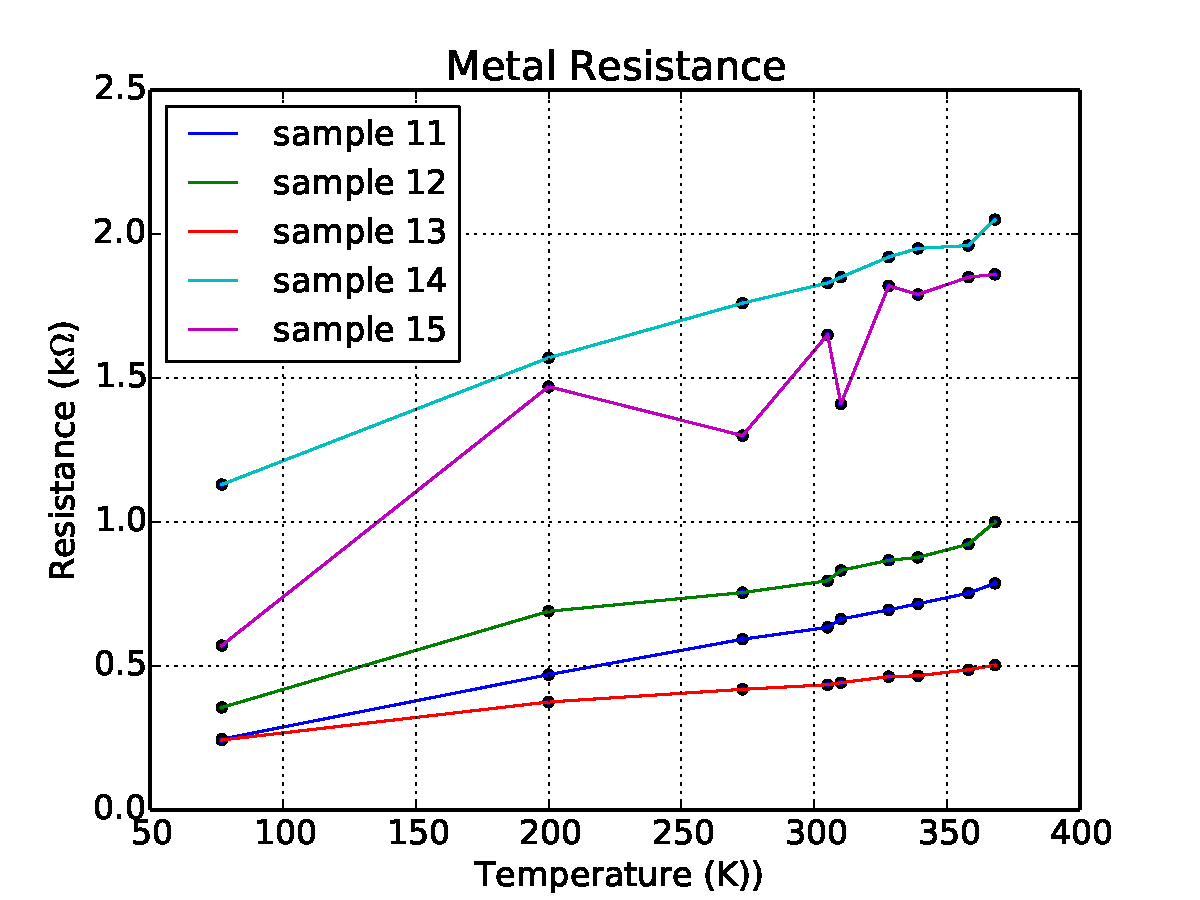
\includegraphics[width=325pt]{data/metal_full.pdf}
\caption{Plot of the data points for metal measurements}
\label{fig:metal}
\end{figure}

\begin{figure}[H]
\centering
\begin{tabular}{c || c | c | c | c | c | c | c | c | c | c | c}
\specialcell{Temperature \\ ($\degree$C)} & -73 & 0 & 23 & 35 & 44 & 53 & 64 & 73 & 83 & 95 & 100 \\ \hline
\specialcell{Resistance \\ k$\Omega$} & 228 & 9.70 & 3.55 & 2.45 & 1.61 & 1.13 & 0.70 & 0.50 & 0.35 & 0.24 & 0.20 \\ \hline
\end{tabular}
\caption{Data recorded for semiconductor (Germanium) heating and resistance measurements}
\end{figure}

\begin{figure}[H]
\begin{tikzpicture}
\node at (5,5) {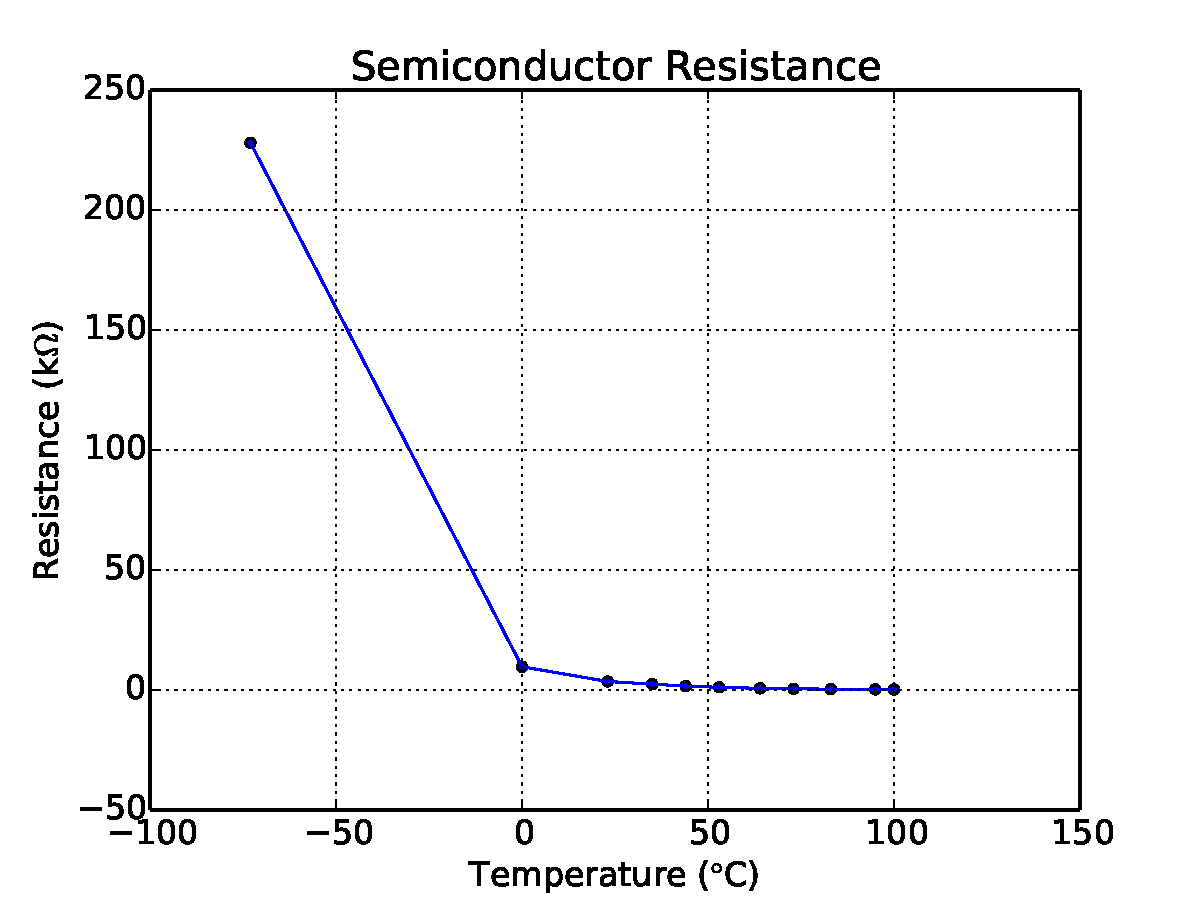
\includegraphics[width=325pt]{data/semi_full.pdf}};
\node at (15,5) {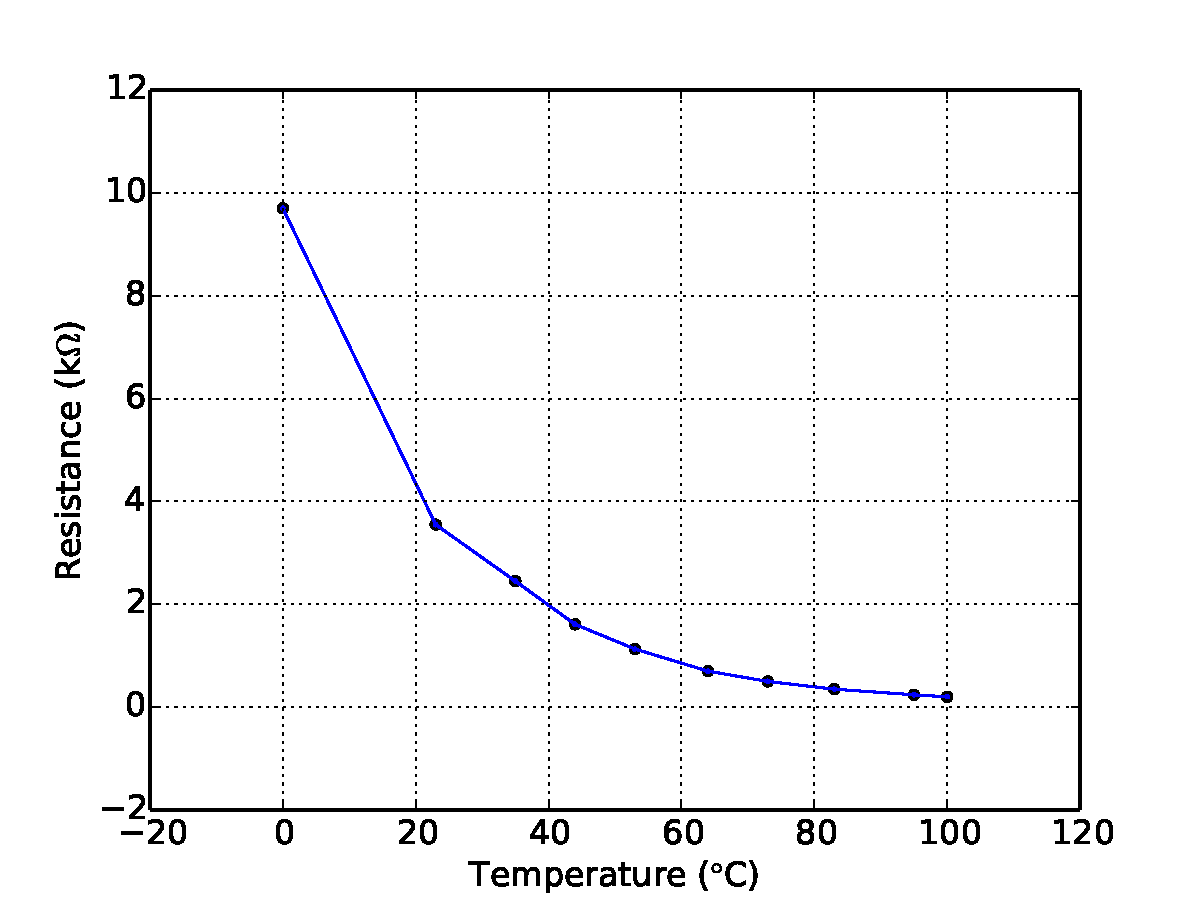
\includegraphics[width=250pt]{data/semi_part.pdf}};
\draw (4,2.5) rectangle (8.2,3.2);
\draw (8.2,3.2) -- (11.7,7.5);
\draw (8.2,2.5) -- (11.7,3);
\end{tikzpicture}
\caption{Plot of the data for Semiconductor heating}
\label{fig3}
\end{figure}


\begin{figure}[H]
\centering
\begin{tabular}{c || c | c | c | c | c | c | c | c}
\specialcell{Temperature \\ ($\degree$C)} & 400 & 450 & 500 & 550 & 600 & 650 & 700 & 750 \\ \hline
\specialcell{Resistance \\ k$\Omega$} & 4.6\e{2} & 2.1\e{2} & 9.2\e{1} & 4.35\e{1} & 1.64 \e{1} & 6.3 & 2.3 & 0.85 \\ \hline
\end{tabular}
\caption{Temperatures and Resistances measured for the salt (NaCl) sample.}
\end{figure}

\begin{figure}[H]
\centering
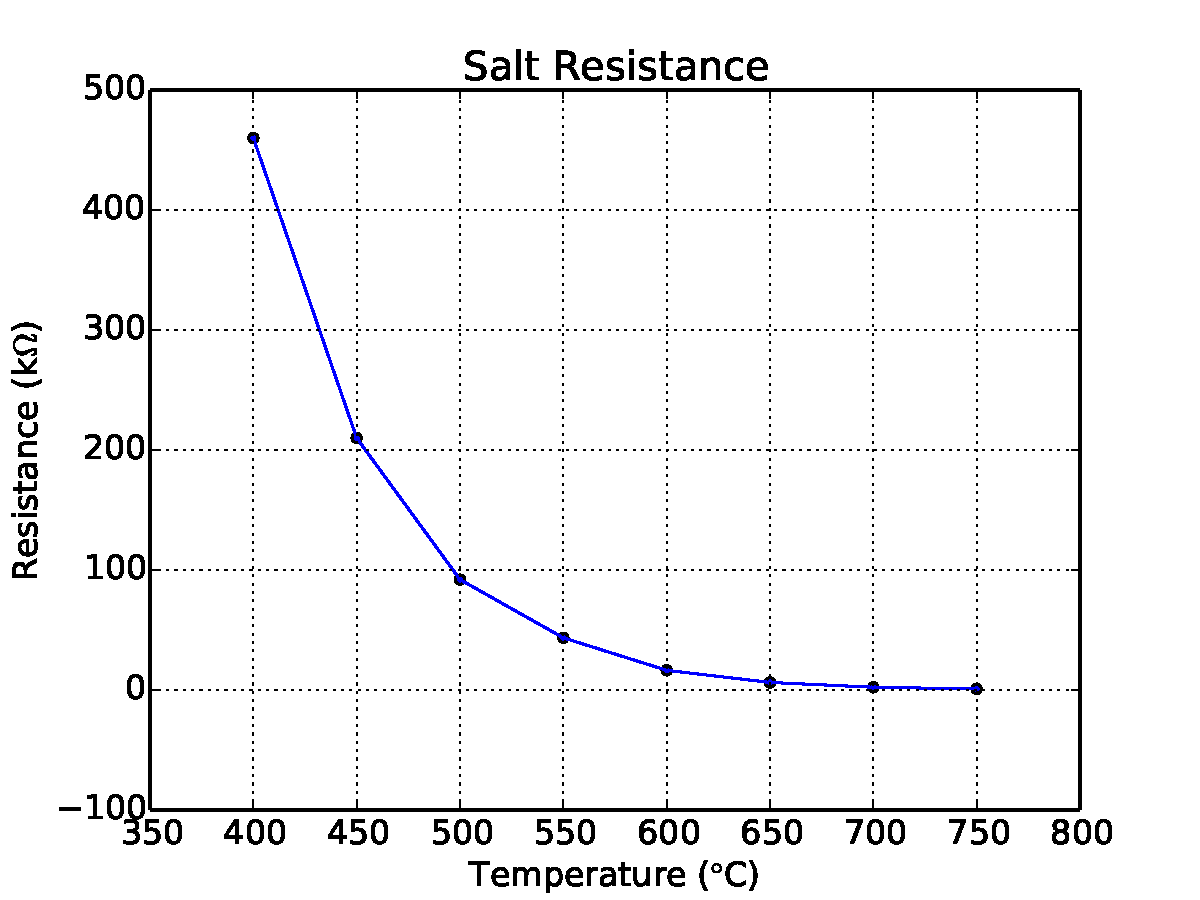
\includegraphics[width=325pt]{data/salt_full.pdf}
\caption{Plot of data for salt measurements}
\end{figure}


\section{Discussion}

\begin{description}[style = nextline]
\item[1) Rank the five (5) specimens in order of purity, and specify $\rho_r$ for each specimen in micro-ohm-cm.]
Using the equation to calculate resistivity on page 3 of the lab manual [2] and picking $T_1 = 77$K and $T_2 = 273$K, we get the following results,
\begin{figure}[H]
\centering
\begin{tabular}{c || c | c}
Purity & Sample & \specialcell{$\rho_r$ \\ ($\mu \Omega$-cm)} \\ \hline
1 & sample 11 & 0.766 \\ \hline
2 & sample 15 & 0.866 \\ \hline
3 & sample 12 & 1.01 \\ \hline
4 & sample 13 & 1.68 \\ \hline
5 & sample 14 & 2.24 \\ \hline 
\end{tabular} 
\caption{Purity rank from highest purity to lowest. i.e. 1 is most pure and 5 is least pure.}
\end{figure}


\item[2) To what precision can you verify Matthiessen's rule? To answer this question, consider how the resistivity changes with temperature for a fixed concentration of impurities, then how the resistivity changes with impurity concentration when the temperature is fixed.]
Looking at all the plots in Figure \textcolor{blue}{\ref{fig:metal}} we can see that $\rho_r$ changes with each line as the impurity concentrations change. However $\rho_{th}$ remains the same across the samples; this means that our slopes should be the same at low temperatures. Now using the data for resistance at 77K and 200K for each metal sample, we can calculate slopes. With five different slopes we can calculate a standard deviation $\sigma$ and a standard error $\alpha = \sigma/\sqrt{n}$. This standard error will tell us the precision of our five slopes, $\rho_{th}$. After calculations we get $3.3 \pm 1.0\, m\Omega/K$. Thus our precision of Matthiessen's rule is $1.0/3.3 = 30\%$. 

\item[3) Would you expect $\rho$ to increase or decrease as T is increased through the melting point? Why?]
The resistivity will increase. This is because it is much harder for electrons to move through a material in the liquid phase rather than a solid phase. In the liquid phase, atoms move around a lot, and as a result, hinder the effectiveness of the electrons to make it across a material without running into something.

\item[4) If you dope a metal A with another metal B where $\rho_B < \rho_A$, do you expect the resistivity of the alloy to increase or decrease? Why?]
Assuming metal A is 100\% pure. Adding another metal B will increase the total resitivity even if $\rho_B < \rho_A$. This is because diffusing the new metal B in A will create lots of defects in the alloy which makes it harder for electrons to move around thus causing resistivity to go up.

\item[5) Plot ln (G) versus 1/T for the semiconducting sample studied in this lab.]
Note the y axis units here. In the lab manual $\ln{G}$ was plotted with units of $\Omega^{-1}m^{-1}$. However, as we all know you cannot take a natural log of a number that has units because there is no physical meaning behind it; natural logs can only be used with unitless numbers. So I have added a constant. Instead we are plotting $\ln{G/G_0}$ where $G_0 = 1$ and has the same units as $G$. Thus there should be no units on the y axis of this plot.

\begin{figure}[H]
\centering
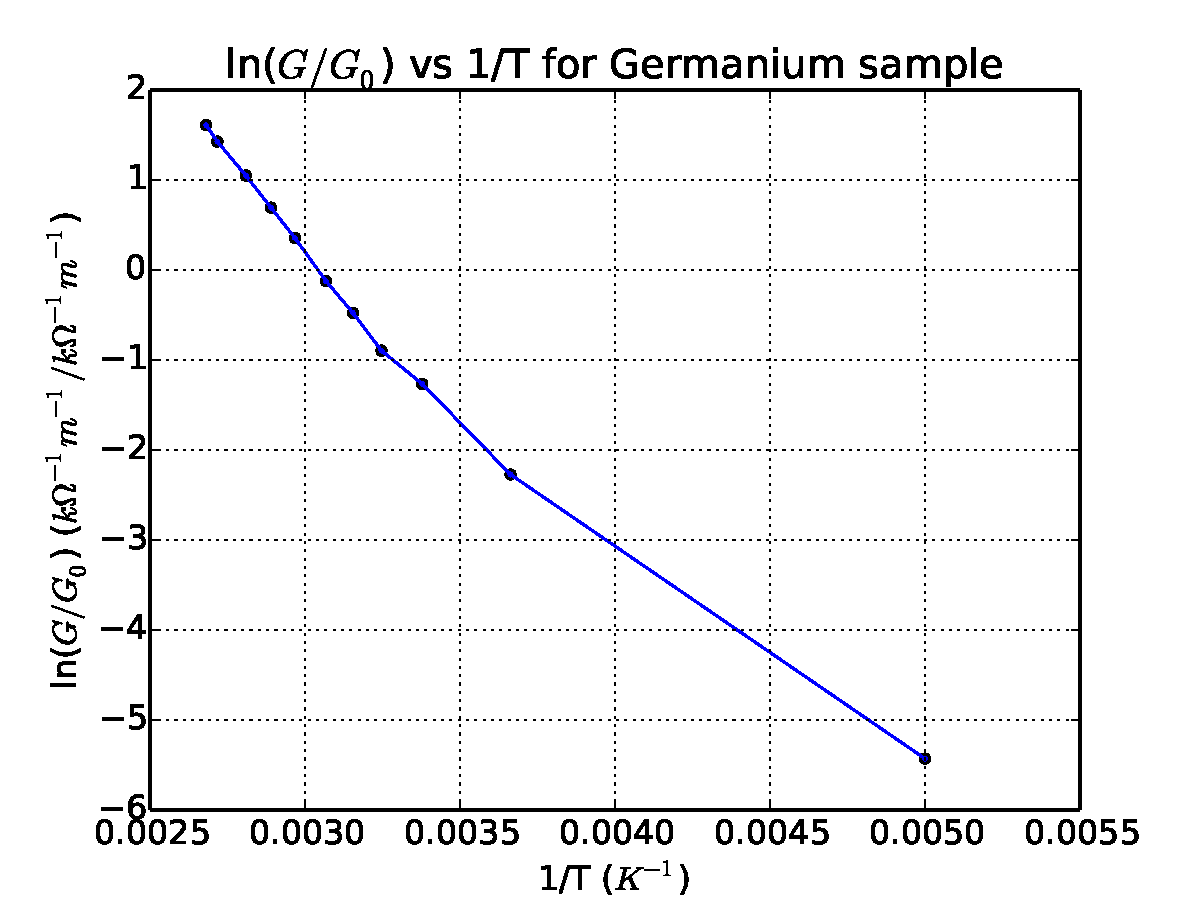
\includegraphics[width=325pt]{data/semi_full_eg.pdf}
\caption{Plot of the natural log of conductance vs inverse temperature for a Germanium semiconductor}
\end{figure}

\item[6) Over what temperature range, if any, does your sample behave as an intrinsic semiconductor?]
Looking at the plot above, the germanium sample does behave like an intrinsic semiconductor at temperatures higher than about room temperature. At cold temperatures of $0\degree$C and $-73\degree$C the sample tends to lose its intrinsic semiconductor behavior. However at temperatures from $23\degree$C to $100\degree$C the sample does show intrinsic semiconductor behavior.

\item[7) What is the energy gap for your sample? Compare with published literature values and cite your sources.]

According to [4], the energy band gap for Germanium is 0.67 eV (at 302K). According to the lab manual [2], the slope of figure 8 should be $-E_g/2k$. Therefore $E_g = -2k(\text{slope})$ where k is boltzmann's constant. Using linear regression and fitting a line to the data in the intrinsic in figure 8, a slope of $-4.42\e{3} K^{-1}$ was calculated with a R value of 0.9997. This corresponds to an $E_g = 0.77$eV. This corresponds to a percent error of 15\%.

\item[8) Predict the resistance at 150$\degree$C of your sample.]

After doing a linear fit on the plot in figure 8, the slope and intercept were calculated to be -3.05\e{4} and 9.371. Using this data we find that:

\begin{align*}
y = mx + b = \frac{-4.42\e{3}}{150\degree\text{C} + 273} + 9.371 = -1.08
\end{align*}
We also know from figure 8 that the y axis corresponds to $\ln{G/G_0}$ where $G_0 = 1$.
\begin{align*}
y = \ln{G/G_0} \Rightarrow -1.08 = ln{G/G_0} \Rightarrow \me^{-1.08} = \frac{G}{G_0} \Rightarrow G = 0.340 \Rightarrow R = 1/G = 2.94\text{k}\Omega.
\end{align*}

\item[9) Plot ln (G) versus 1/T for the insulator sample studied in this lab.]
See below plot.

\begin{figure}[H]
\centering
\begin{tikzpicture}
\node at (5,5) {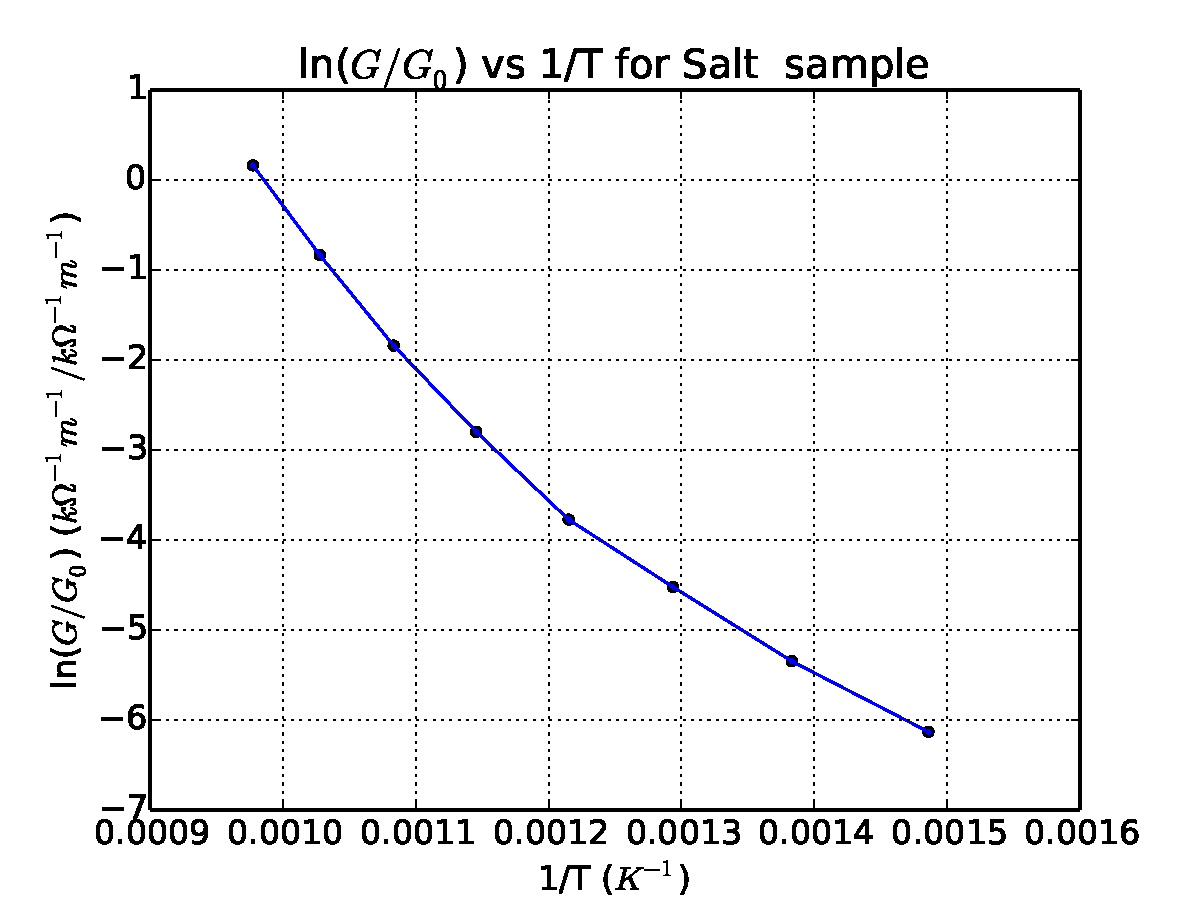
\includegraphics[width=325pt]{data/salt_full_eg.pdf}};
\draw [dashed,color=red](4.7,1.6) -- (4.7,8);
\end{tikzpicture}
\caption{Plot of the natural log of conductance vs inverse temperature for salt (NaCl). Dashed red line indicates a change in slope}
\end{figure}

\item[10) What is the temperature corresponding to the change in slope of the ln (G) vs 1/T plot? If you don't observe any change in slope, what does that mean?]
%% FIGURE 3 description in lab manual.
Looking at figure 9 the slope change occurs roughly in the middle of the graph as indicated by the red line. This corresponds to a temperature of $550\degree$C. If the slope does not become steeper afterwards then that means no Shottky defects ended up forming.

\item[11) From your plot determine both $E_m$ and $W$ in eV.]
From the lab manual [2] we know that the slope on the upper part of the graph in figure 9 should be equal to $-(E_m + [W/2])/k$ and the slope on the bottom part of the graph is equal to $-E_m/k$ where $k$ is boltmann's constant. Using linear regression on both parts of the plot in figure 9, slopes of -8.73\e{4}$K^{-1}$ and -1.76\e{5}$K^{-1}$ were calculated.

\begin{align*}
E_m =& -\frac{\text{slope}}{k} = -\frac{-8.73\e{4}}{1.38\e{-23}} = 6.33\e{27} \text{J} =  \\
W =& -2(\text{slope}*k + E_m) = -2(-1.76\e{5}*1.38\e{-23} + 6.33\e{27}) = 1.27\e{28} \text{J} = 
\end{align*} 

\item[12) Do you think that conductivity measurements could be used as an index of purity in ionic crystals? Discuss.]
Yes. Having lots of defects in a material makes it much harder for electrons to move around causing low conductivity measurements. The purer the crystal, the easier it is for electrons to move through the material and thus would have a higher conductivity. So it is very reasonable to say that conductivity can be used as an indirect way to measure pureness of materials.

\end{description}

%----------------------------------------------------------------------------------------
%	SECTION 4
%----------------------------------------------------------------------------------------

\section{Conclusions}
As a result of this investigation, the following conclusions can be drawn.
\begin{enumerate}
\item We confirmed the energy band gap of Germaniam to within 15\% error using our experimental setup.
\item For insulators, resistance goes down exponentially with an increase in temperature. Similarly semiconductors have their resistance go down but not as drastically as insulators with an increase in temperature. For metals, resistance goes up with an increase in temperature.

\end{enumerate}

%----------------------------------------------------------------------------------------
%	SECTION 5
%----------------------------------------------------------------------------------------

\section{References}
\begin{enumerate}
\item James F. Shackelford, Introduction to Materials Science for Engineers, Seventh Edition, Pearson Higher 
Education, Inc., Upper Saddle River, New Jersey (2009).
\item Gronsky, Ron. Lab 06 Manual: Electronic Properties of Materials. Berkeley: Ronald Gronsky, 2014. Web.
\item Justin Chen and Sarah Hull. E45. Lab sec 103.
\item Streetman, Ben G.; Sanjay Banerjee (2000). Solid State electronic Devices (5th ed.). New Jersey: Prentice Hall. p. 524. ISBN 0-13-025538-6.
\end{enumerate}

%----------------------------------------------------------------------------------------
%	SECTION 6
%----------------------------------------------------------------------------------------

% Nothing right now

%----------------------------------------------------------------------------------------
%	BIBLIOGRAPHY
%----------------------------------------------------------------------------------------

\bibliographystyle{apalike}

\bibliography{sample}

%----------------------------------------------------------------------------------------


\end{document}

